
\documentclass[11pt]{article}
\usepackage{UF_FRED_paper_style}
\usepackage{listings}
\usepackage{hyperref}
\hypersetup{
	colorlinks=true,
	linkcolor=blue,
	filecolor=blue,      
	urlcolor=blue,
	citecolor=cyan,
}

%% ===============================================
%% Setting the line spacing (3 options: only pick one)
% \doublespacing
% \singlespacing
\onehalfspacing
%% ===============================================

\setlength{\droptitle}{-5em} %% Don't touch

% %%%%%%%%%%%%%%%%%%%%%%%%%%%%%%%%%%%%%%%%%%%%%%%%%%%%%%%%%%
% SET THE TITLE
% %%%%%%%%%%%%%%%%%%%%%%%%%%%%%%%%%%%%%%%%%%%%%%%%%%%%%%%%%%

% TITLE:
\title{COMSM0104: Web Technologies 2019 \\Final Assignment Report}

% AUTHORS:
\author{Tao Xu\\% Name author
	\href{mailto:si19010@bristol.ac.uk}{\texttt{si19010@bristol.ac.uk}} %% Email author 1 
	\and Yinan Yang\\% Name author
	\href{mailto:ff19085@bristol.ac.uk}{\texttt{ff19085@bristol.ac.uk}} %% Email author 2
}

% DATE:
\date{\today}

% %%%%%%%%%%%%%%%%%%%%%%%%%%%%%%%%%%%%%%%%%%%%%%%%%%%%%%%%%%
% %%%%%%%%%%%%%%%%%%%%%%%%%%%%%%%%%%%%%%%%%%%%%%%%%%%%%%%%%%
\begin{document}
	% %%%%%%%%%%%%%%%%%%%%%%%%%%%%%%%%%%%%%%%%%%%%%%%%%%%%%%%%%%
	% %%%%%%%%%%%%%%%%%%%%%%%%%%%%%%%%%%%%%%%%%%%%%%%%%%%%%%%%%%
	% ABSTRACT
	% %%%%%%%%%%%%%%%%%%%%%%%%%%%%%%%%%%%%%%%%%%%%%%%%%%%%%%%%%%
	% %%%%%%%%%%%%%%%%%%%%%%%%%%%%%%%%%%%%%%%%%%%%%%%%%%%%%%%%%%
	{\setstretch{.8}
		\maketitle
		% %%%%%%%%%%%%%%%%%%
		\begin{abstract}
			% CONTENT OF ABS HERE--------------------------------------
			
			Our two-person team consists of Tao Xu (si19010) and Yinan Yang (ff19085). Due to environmental influences, we used a remote collaboration model via GitHub to co-develop this project.
			
			We have created a website that generates resumes. Our website is based on Vue's front-end technical architecture, taking advantage of Vue's MVVM, the Model-View- ViewModel, we have done it to componentize the front-end development.
			
			% END CONTENT ABS------------------------------------------
			\noindent
			\textit{\textbf{Keywords: }%
				Vue; SQLite.} \\ %% <-- Keywords HERE!
			\noindent
			% \textit{\textbf{JEL Classification: }%
			% Q12; C22; D81.} %% <-- JEL code HERE!
			
		\end{abstract}
	}
	
	% %%%%%%%%%%%%%%%%%%%%%%%%%%%%%%%%%%%%%%%%%%%%%%%%%%%%%%%%%%
	% %%%%%%%%%%%%%%%%%%%%%%%%%%%%%%%%%%%%%%%%%%%%%%%%%%%%%%%%%%
	% BODY OF THE DOCUMENT
	% %%%%%%%%%%%%%%%%%%%%%%%%%%%%%%%%%%%%%%%%%%%%%%%%%%%%%%%%%%
	% %%%%%%%%%%%%%%%%%%%%%%%%%%%%%%%%%%%%%%%%%%%%%%%%%%%%%%%%%%
	
	% --------------------
	\section{Introduction}
	% --------------------
	
	We have created a website that generates resumes called Simple Resume Maker. The website provides basic user registration and login functionality. Once logged in, the user can edit the resume template provided on the website on the web page and download a .pdf version of the resume.
	
	We try to simulate the user experience of editing documents online so that what the user sees is what they get. What would otherwise be a cumbersome formatting process is made easier with different CSS. This addresses the initial point we made in designing the product, which was to make things easier.
	
	In building this site, we used the VUE framework, which is a progressive framework for building user interfaces. 
	
	\begin{center}
		\fbox{\shortstack[l]{
				Unlike other monolithic frameworks, Vue is designed from the ground up to be\\ incrementally adoptable. The core library is focused on the view layer only, and\\ is easy to pick up and integrate with other libraries or existing projects. On the\\ other hand, Vue is also perfectly capable of powering sophisticated Single-Page\\ Applications when used in combination with modern tooling and supporting\\ libraries.\\
				----- Official development documentation from Vue
			}}
		
	\end{center}

	
	\subsection{Project setup}
		npm install
	\subsection{Compiles and hot-reloads for development}
	npm run serve
	\subsection{Compiles and minifies for production}
	npm run build
	\subsection{Lints and fixes files}
	npm run lint
	\subsection{Start the server}
	npm start
	\subsection{Start the server}
	See \href{https://cli.vuejs.org/config/}{Configuration Reference}.
		
	% --------------------
	\section{Self Evalutation}
	\subsection{Estimation of marks}
\begin{itemize}
	\item A for HTML
	\item A for CSS
	\item A for JS
	\item A for PNG	
	\item A for SVG
	\item A for Server
	\item A for Database
	\item A for Dynamic pages
\end{itemize}
	\subsection{Client Side}
	\subsubsection{HTML}
	\subsubsection{CSS}
	\subsubsection{JS}
	\subsubsection{PNG}
	\subsubsection{SVG}
	In the use of SVG, we have used a variety of ways to construct SVG images to take full advantage of his benefits. We even created SVG  animation on the home page. We will describe this in detail below.
	\begin{itemize}
		\item Basic SVG images\\
		We used tools like Inkscape to draw simple SVG portraits, and since the team has the skills to operate adobe Kit experience, so we are light on SVG production. 
		\begin{figure}[H]
			\centering
			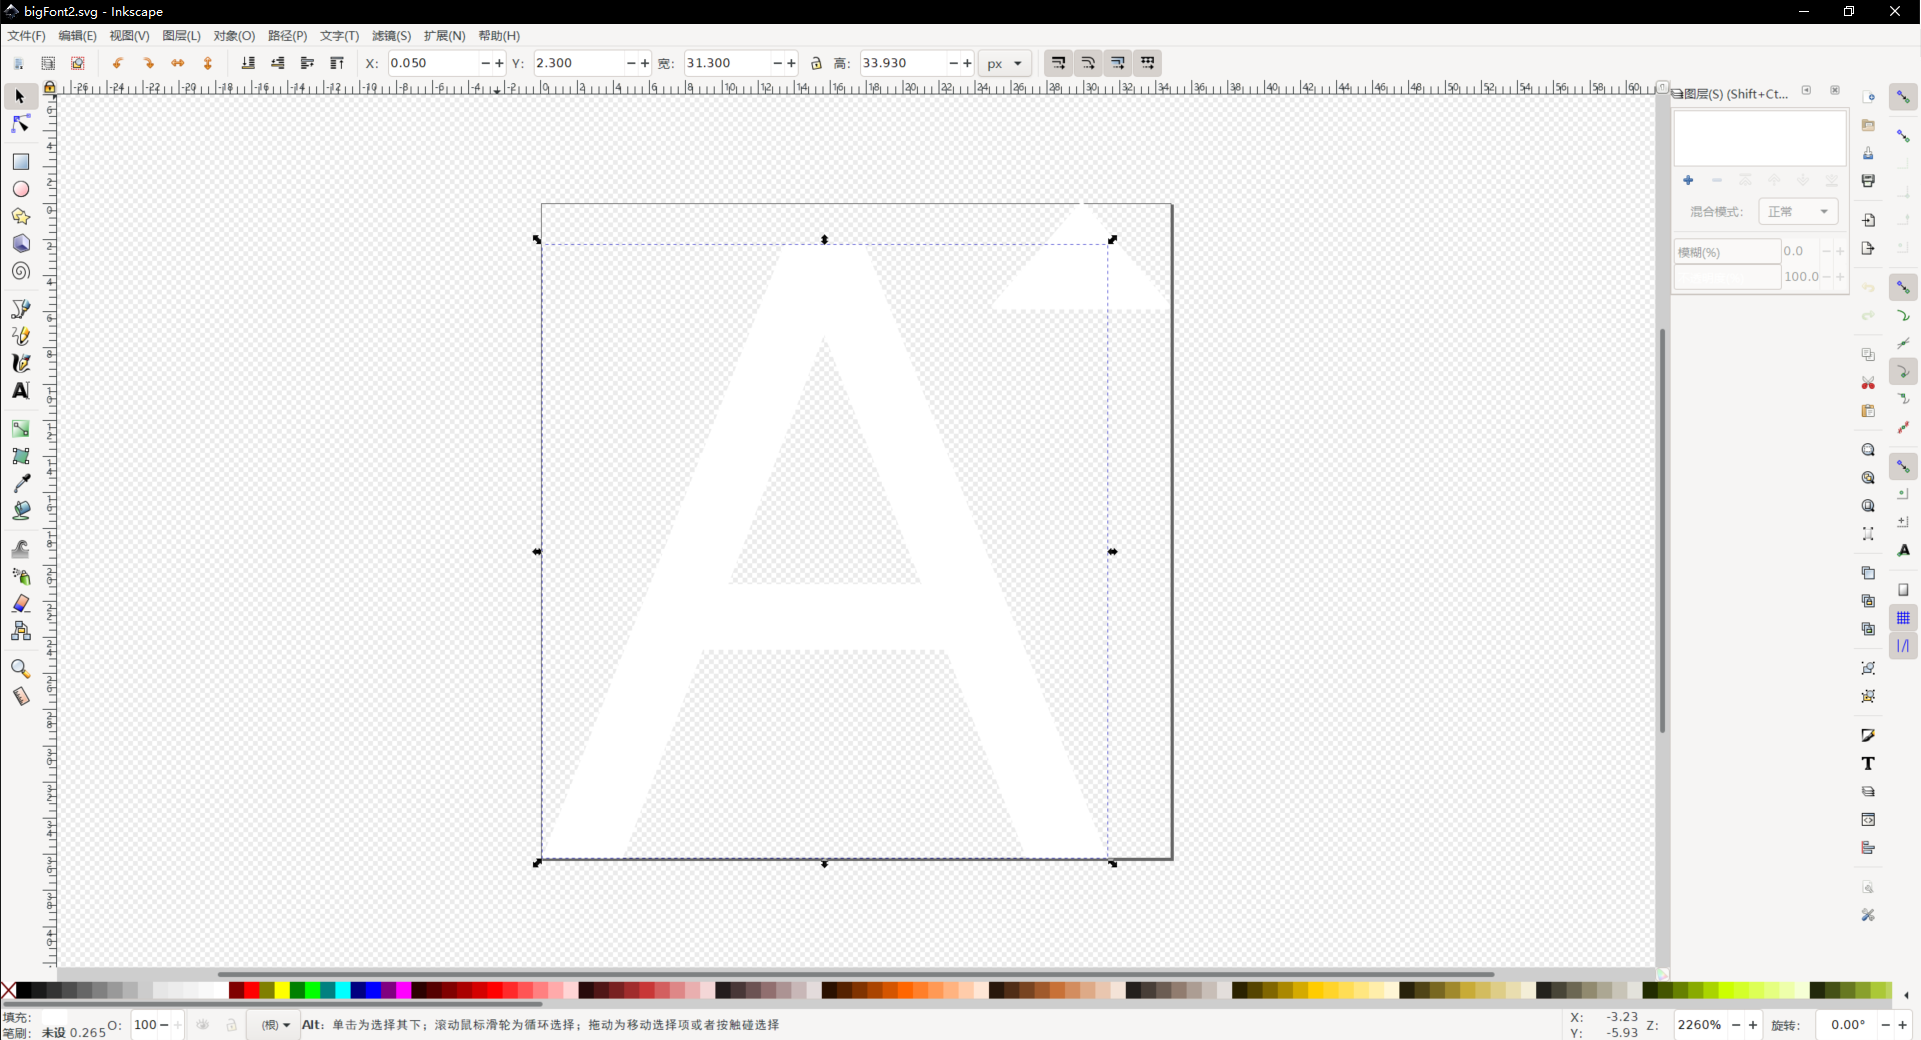
\includegraphics[scale=.3]{figures/svg1.png}
			\caption{Inkscape}
			\label{fig:1}
		\end{figure}
	We used this basic graphical drawing to create 12 buttons, 3 of which are embedded in the page, while the remaining nine are used as Individual components are independent of the elements in the $src/components/button$. We take advantage of the object-oriented component design of the Vue components so that each module is easy to maintain and update later.
	\begin{figure}[H]
		\centering
		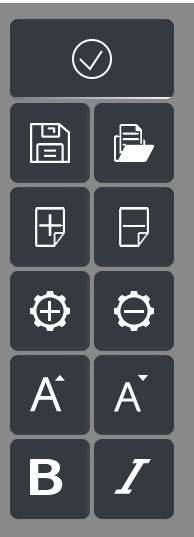
\includegraphics[scale=.3]{figures/buttonBar.png}
		\caption{buttonBar}
		\label{fig:2}
	\end{figure}
	\begin{figure}[H]
	\centering
	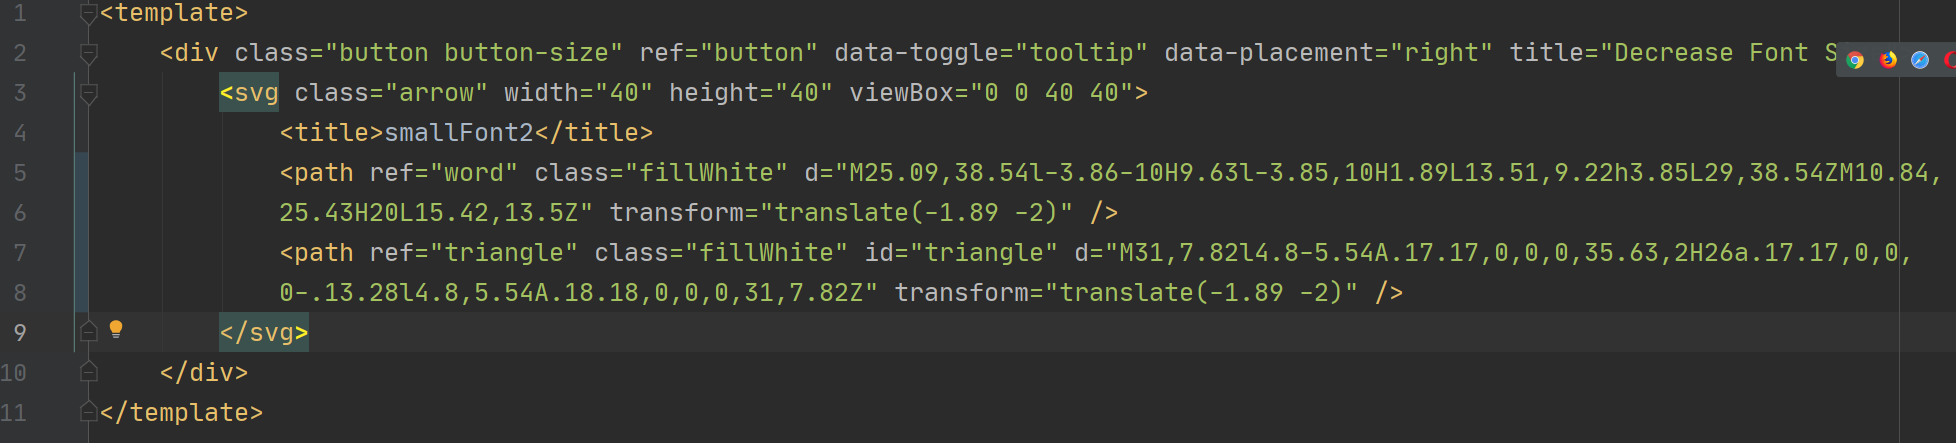
\includegraphics[scale=.3]{figures/smallFontButton.png}
	\caption{smallFontButton}
	\label{fig:3}
\end{figure}
\item SVG-based css animation\\
We were not satisfied with making basic SVG graphics. We created four SVG animations with CSS animation effects. They are the start button on the home page, the continue and new buttons on the user-profile page, and the download button inside CVMaker. The most complex one is the download button, which activates the animation by changing the button's class when clicked. 
\begin{figure}[H]
	\centering
	
\includegraphics[scale=1]{figures/downloadButton.png}
	\caption{downloadButton animation}
	\label{fig:4}
\end{figure}
The download animation is divided into four parts, the first is the flashing of the outer ring, the second is the downward movement of the vertical line in the middle, and the third is the download of The middle arrow pattern becomes a checkmark when finished, and the fourth is the download progress bar at the bottom.
\begin{figure}[H]
	\centering
	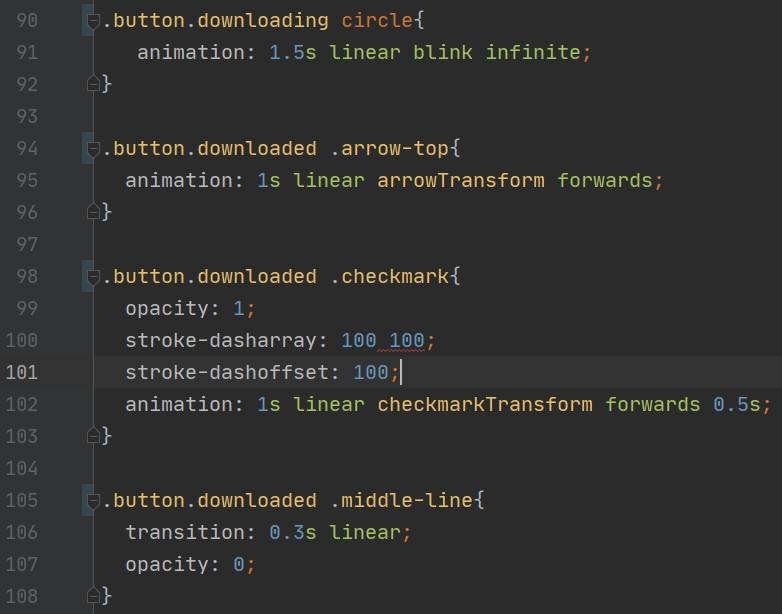
\includegraphics[scale=0.5]{figures/cssAnimation.png}
	\caption{downloadButton animation}
	\label{fig:5}
\end{figure}
\item svg animation based on vue-lottie\\
Of course, doing this will not satisfy our ambition to try the coolest animations. So we introduced the vue-lottie open-source package, which is based on the \href{https://github.com/airbnb/lottie-web}{lottie}. Vue-lottie project vue architecture lottie can be interpreted as an SVG animation interpreter, and he supports the use of SVG in adobe After Effects exports complex animations to a JSON file and then self-rendering through the front-end of the web page to get cool effects.

We've made a dynamic animation on the home page to highlight our theme, which we're sure you've seen.We save the exported animation JSON file that we send to AE in the $src/view/index/assets/animation$ folder.
\begin{figure}[H]
	\centering
	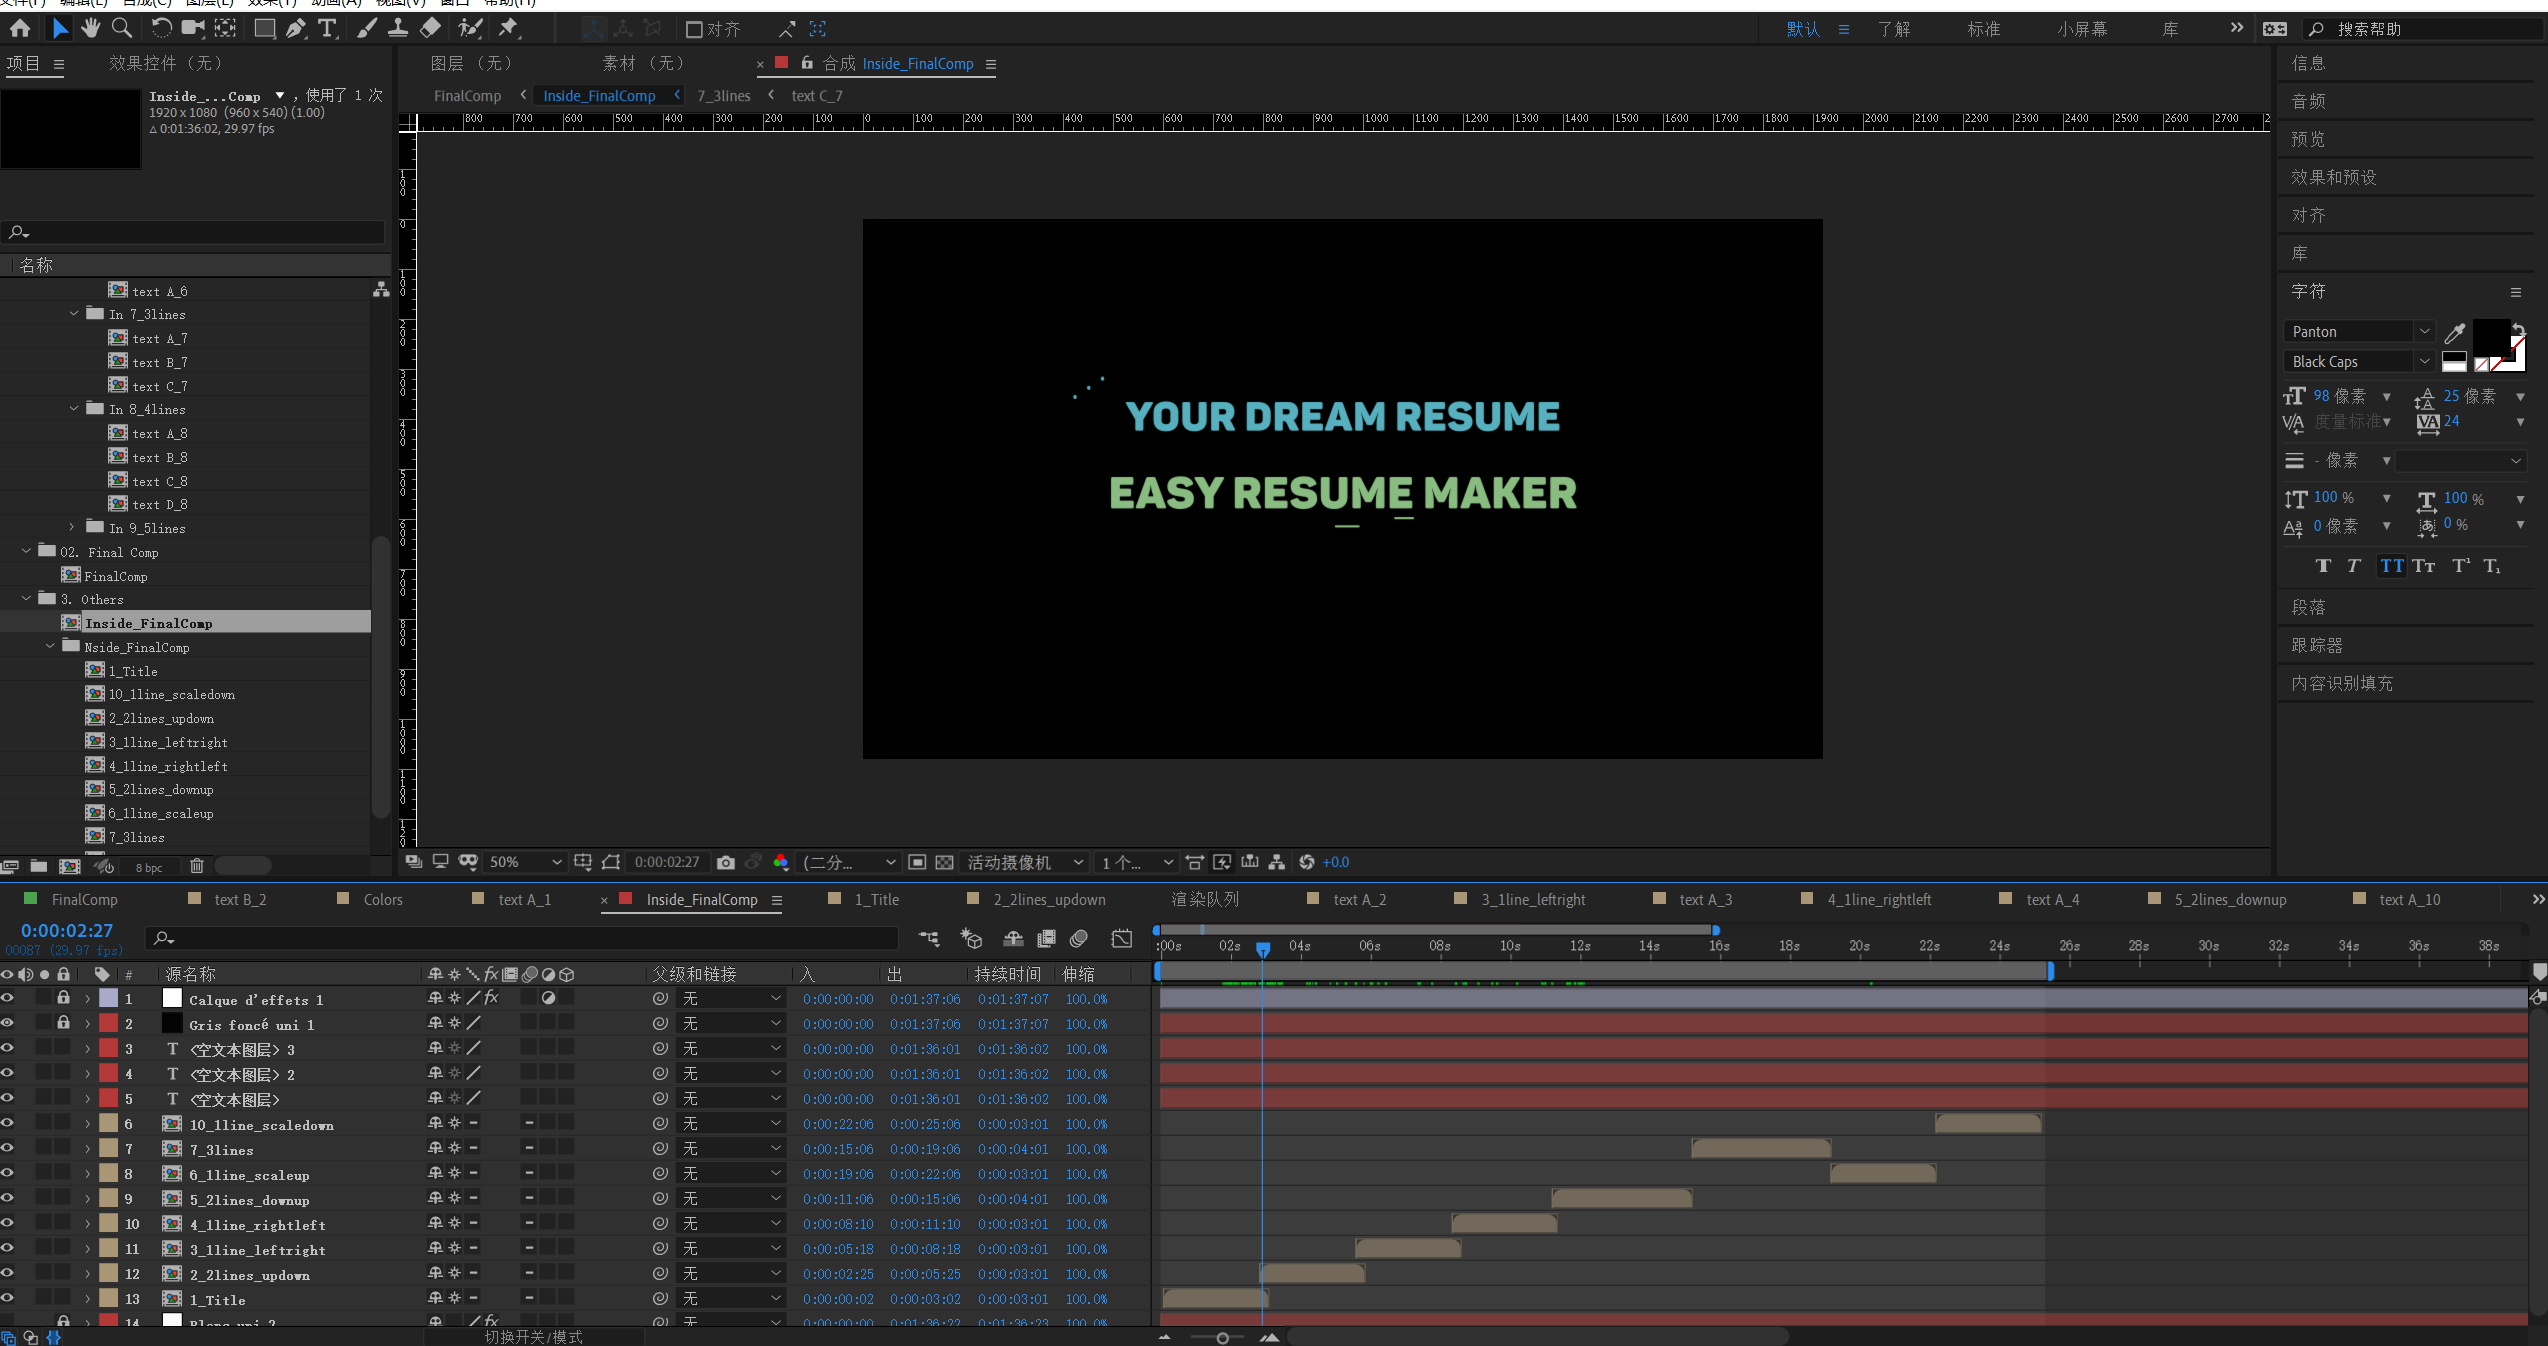
\includegraphics[scale=0.2]{figures/ae.png}
	\caption{After Effect}
	\label{fig:6}
\end{figure}
Since this lottie tool is so new, we think we have made it pretty far ahead of the curve in terms of SVG usage.

	\end{itemize}
	\subsection{Server Side}
	\subsubsection{Server}
	\subsubsection{Database}
	\subsubsection{Dynamic pages}
	
	% --------------------
	% --------------------
	\section{Working practices of the group}
	% --------------------
	

	
	% --------------------
	
	
	
\end{document}